\minisec{Zwei Abbildungen nebeneinander}
%
\texttt{Abbildungen} fallen unter \emph{floating objects} und werden in der \texttt{figure}-Umgebung in den Text eingebunden.
Für mehrere Bilder in einer Abbildung mit jeweils eigener Beschriftung können wir die \texttt{subfigure}-Umgebung verwenden (siehe Abb.~\ref{fig:bsp-subfigure})
%
Abb.~\ref{fig:xkcd-citogenesis} zeigt ein Problem des Zitierens aus Wikipedia. 
Da manche Menschen alles glauben, was in Wikipedia geschrieben steht, stellt dieser Comik aus \url{https://xkcd.com} die Glaubwürdigkeit zumindest ein bisschen in Frage.
Eine Erklärung dazu befindet sich auf \url{https://www.explainxkcd.com/wiki/index.php/978:_Citogenesis}.
Abb.~\ref{fig:logo-fakultät} zeigt das Logo unserer Fakultät.
%
\begin{figure}[ht]
  \begin{subfigure}[t]{0.50\textwidth}
   \centering
   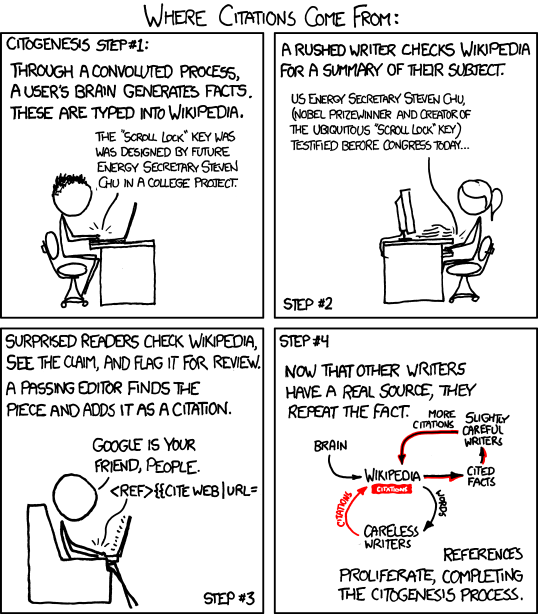
\includegraphics[width=7cm]{citogenesis}
   \caption[Zitierproblematik]{Ein Glaubwürdigkeitsproblem mancher Artikel in Wikipedia (Quelle: \url{https://xkcd.com/978/})    \label{fig:xkcd-citogenesis}}
  \end{subfigure}
\hfill
  \begin{subfigure}[t]{0.45\textwidth}
   \centering
   \includegraphics[width=0.85\textwidth]{tuw-bui-logo-2022}
   \caption{Logo der Fakultät für Bau- und Umweltingenieurwesen der TU Wien \label{fig:logo-fakultät}}
  \end{subfigure}
\caption{Beispiel einer \texttt{subfigure}-Umgebung \label{fig:bsp-subfigure}}
\end{figure}
%


\minisec{Matrix-Schreibweise}
%
Die Steifigkeitsmatrix sowie die Nachgiebigkeitsmatrix des Materials sind mit Bezug auf die Materialhauptrichtungen $L$-$R$-$T$ gegeben (siehe~\eqref{Glg:sigma} bis \eqref{Glg:D-matrix}).

Gesucht ist der Verzerrungstensor $\varepsilon$ im globalen Koordinatensystem $X,Y,Z$ sowie die Koordinaten der Eckpunkte in der verformten Lage (angegeben in [\si{mm}] auf 3~Dezimalstellen) unter der Annahme einer linearisierten Elastizitätstheorie.

\begin{equation}
\boldsymbol{\sigma}
=
\left(
   \begin{array}{c}
      \sigma_{xx} \\
      \sigma_{yy} \\
      \sigma_{zz} \\
      \sigma_{xy} \\
      \sigma_{yz} \\
      \sigma_{zx} \\
   \end{array}
\right)
=
\left(
   \begin{array}{c}
      1x{,}y \\
      1{,}xy \\
      2{,}xy \\
      3{,}xy \\
      0      \\
      0      \\
   \end{array}
\right)
\si{N/mm^2}
\label{Glg:sigma}
\end{equation}

\begin{equation}
\textbf{C}_{(LRT)}
=
\left(
\begin{array}{rrrccc}
\num{15500} & 489 & 274 & 0   & 0  & 0  \\
      & 844 & 162 & 0   & 0  & 0  \\
      &     & 632 & 0   & 0  & 0  \\
      &     &     & 700 & 0  & 0  \\
      &     &     &     & 60 & 0  \\
   \multicolumn{2}{l}{\text{symm.}}  
            &     &     &    & 650 \\
\end{array}
\right)
%
\cdot
%
\left(
   \begin{array}{c}
      \epsilon_{xx} \\
      \epsilon_{yy} \\
      \epsilon_{zz} \\
      \epsilon_{xy} \\
      \epsilon_{yz} \\
      \epsilon_{zx} \\
   \end{array}
\right)
=
\left(
   \begin{array}{r}
      \num{12,70} \\
      \num{1,27}  \\
      \num{2,27}  \\
      \num{3,27}  \\
      \multicolumn{1}{c}{0}     \\
      \multicolumn{1}{c}{0}     \\
   \end{array}
\right)
\label{Glg:C-matrix}
\end{equation}

\begin{equation}
\textbf{D}_{(LRT)}
=
\left(
   \begin{array}{rrrccc}
\num{6,595} &  \num{-3,441} &  \num{-1,977} &  0  &  0  & 0 \\
            & \num{126,411} & \num{-30,911} &  0  &  0  & 0 \\
            &               & \num{167,008} &  0  &  0  & 0 \\
            &               &               & \num{142,857} &  0  &  0  \\
            &               &               &    & \num{1666,667}  &  0  \\
   \multicolumn{2}{l}{\text{symm.}} &       &    &      & \num{153,846}  \\
\end{array}
\right)
\cdot \SI{e-5}{mm^2/N}
\label{Glg:D-matrix}
\end{equation}



\minisec{Beispiel für xfrac-Paket}
%
Dieses Paket verwendet den Befehl \textbackslash{}sfrac\{\}\{\} im Text
\sfrac{3}{4} oder in einer Formel $\sfrac{3}{4}$.

\minisec{Beispiele für den Einsatz des siunitx-packages}
Eine Verwendungsmöglichkeit ist die richtige Anzeige von Zahlen:
%
\begin{itemize} 
  \item als Einzelzahl: \num{12345678,9202}
  \item als Bereich von Zahlen: \numrange{12,3}{14,7} 
  \item als Liste von Zahlen: 
                      \numlist[list-final-separator={ und }]{12,3;13,5;14,7}
\end{itemize}
%
oder die richtige Darstellung von Einheiten (unabhängig ob im Paragraph- oder Math-Modus):
%
\begin{itemize} 
  \item Paragraphmodus: \si{\kilo\newton\per\meter}, \si{kN/m^2}
  \item Mathematikmodus:  $\si{\kilo\newton\per\meter}$, $\si{kN/m^2}$
\end{itemize}
%
oder die richtige Darstellung von Zahlen mit Einheiten:
%
\begin{itemize} 
  \item als Einzelzahl: \SI{12345678,92}{kNm}
  \item als Winkel: \ang{10}, \ang{12.3} oder \ang{12;3;5}
  \item als Bereich von Zahlen: \SIrange{12,3}{14,7}{\%} oder 
          \SIrange[range-units = single]{12,3}{14,7}{\%}
  \item als Liste von Zahlen: 
        \SIlist[list-final-separator={ und }]{12,3;13,5;14,7}{\kilogram/m^2}
\end{itemize}
%

\minisec{Beipiele für Abkürzungen samt zugehörigem Verzeichnis}

Das Programm \ac{rlt} wurde in Zusammenarbeit mit der \ac{obv} erstellt, berücksichtigt die deutsche \ac{abbv} -- von mehreren \aclp{abbv} -- und berechnet \ac{lzk}.

Nochmals:
Das Programm LZKB wurde in Zusammenarbeit mit der \ac{obv} erstellt, berücksichtigt die deutsche \ac{abbv} -- von mehreren \acp{abbv} -- und berechnet \ac{lzk}.

\printacronyms[name=Abkürzungen]



\minisec{Beispiel für den Einsatz des tabularx-packages}
Dieses Paket bietet die Möglichkeit der automatischen Anpassung der Spaltenbreite auf eine Gesamtbreite der Tabelle (siehe Tab.~\ref{tab:test}).


\begin{table}[h]
\caption{Ergebnisse der schriftlichen Prüfung \label{tab:test}}
   \begin{tabularx}{\textwidth}{@{}lccX@{}}
   \toprule
   Name & Entwurf     & Pläne       & Anmerkung    \\
   \midrule
   Mayer    & \SI{60}{\%} & \SI{60}{\%} & 
      Funktionalle Umsetzung mit hinreichender Routine. Konstruktive Darstellung speziell im Dachbereich nicht nachvollziehbar. \\
   Müller   & \SI{20}{\%} & \SI{30}{\%} & 
      In allen Teilbereichen sehr detailierte Konzeption, allerdings fehlt die planliche Umsetzung, sodass aufgrund des fehlenden Informationsgehalts keine positive Beurteilung möglich ist. \\
   Schmidt  & \SI{90}{\%} & \SI{90}{\%} & 
      In allen Prüfungsabschnitte routinierte Darstellung und planliche Umsetzung. Die Nachvollziehbarkeit ist in allen Teilabschnitten gegeben. \\
   \bottomrule
   \end{tabularx}
\end{table}




\minisec{Beispiel für den Einsatz der longtable- und multirow-packages}

\begin{longtable}{@{}l*{3}{S[table-format=2.2]}@{}}
\caption{Messwerte der bauphysikalischen Untersuchung \label{tab:bauphysik}}
\\ \toprule
Datum & {Mittel [\si{\degreeCelsius}]} & {Min [\si{\degreeCelsius}]} & {Max [\si{\degreeCelsius}]}
\\ \midrule
\endfirsthead
\caption{Messwerte der bauphysikalischen Untersuchung (Fortsetzung)}
\\ \toprule
Datum & {Mittel [\si{\degreeCelsius}]} & {Min [\si{\degreeCelsius}]} & {Max [\si{\degreeCelsius}]}
\\ \midrule
\endhead
%
  \midrule
  \multicolumn{4}{r}{{Continued on next page}} 
  \\ \bottomrule
\endfoot
%
  \bottomrule
\endlastfoot
06-Jul-2016 & 24,6 & 20,9 & 25,0 \\
07-Jul-2016 & 24,82 & 24,50 & 25,30 \\
08-Jul-2016 & 24,58 & 24,30 & 25,10 \\
09-Jul-2016 & 24,58 & 24,40 & 24,80 \\
10-Jul-2016 & 24,53 & 24,40 & 24,90 \\
11-Jul-2016 & 24,55 & 24,20 & 25,00 \\
12-Jul-2016 & 24,55 & 24,40 & 24,70 \\
13-Jul-2016 & 24,55 & 24,40 & 24,70 \\
14-Jul-2016 & 25,02 & 24,50 & 25,40 \\
15-Jul-2016 & 25,22 & 24,80 & 25,50 \\
16-Jul-2016 & 25,45 & 25,30 & 25,70 \\
17-Jul-2016 & 25,35 & 24,80 & 25,70 \\
18-Jul-2016 & 25,29 & 24,80 & 25,70 \\
19-Jul-2016 & 24,83 & 24,60 & 25,10 \\
20-Jul-2016 & 24,73 & 24,60 & 25,00 \\
21-Jul-2016 & 24,68 & 24,50 & 24,90 \\
22-Jul-2016 & 24,70 & 24,60 & 25,00 \\
23-Jul-2016 & 24,72 & 24,60 & 25,00 \\
24-Jul-2016 & 24,81 & 24,60 & 25,00 \\
25-Jul-2016 & 24,74 & 24,50 & 25,00 \\
26-Jul-2016 & 24,70 & 24,60 & 24,80 \\
27-Jul-2016 & 24,72 & 24,50 & 25,00 \\
28-Jul-2016 & 24,66 & 24,50 & 24,90 \\
29-Jul-2016 & 24,66 & 24,50 & 24,80 \\
30-Jul-2016 & 24,69 & 24,60 & 24,80 \\
31-Jul-2016 & 24,77 & 24,70 & 25,00 \\
01-Aug-2016 & 24,72 & 24,40 & 25,00 \\
02-Aug-2016 & 24,64 & 24,50 & 24,90 \\
03-Aug-2016 & 24,73 & 24,60 & 25,00 \\
04-Aug-2016 & 24,74 & 24,60 & 24,80 \\
05-Aug-2016 & 24,76 & 24,60 & 25,20 \\
06-Aug-2016 & 25,30 & 24,80 & 25,70 \\
07-Aug-2016 & 25,10 & 24,70 & 25,60 \\
08-Aug-2016 & 25,06 & 24,80 & 25,50 \\
09-Aug-2016 & 24,89 & 24,70 & 25,20 \\
10-Aug-2016 & 25,52 & 25,00 & 25,80 \\
11-Aug-2016 & 25,60 & 25,30 & 25,80 \\
12-Aug-2016 & 25,81 & 25,60 & 26,00 \\
13-Aug-2016 & 25,95 & 25,50 & 26,30 \\
14-Aug-2016 & 25,79 & 25,40 & 26,30 \\
15-Aug-2016 & 25,47 & 25,20 & 25,90 \\
16-Aug-2016 & 25,36 & 25,10 & 25,90 \\
17-Aug-2016 & 25,33 & 25,10 & 25,80 \\
18-Aug-2016 & 25,42 & 25,00 & 25,90 \\
19-Aug-2016 & 25,36 & 25,00 & 25,70 \\
20-Aug-2016 & 25,37 & 25,00 & 25,80 \\
21-Aug-2016 & 25,38 & 25,10 & 25,70 \\
22-Aug-2016 & 25,88 & 25,60 & 26,20 \\
23-Aug-2016 & 25,85 & 25,10 & 26,70 \\
24-Aug-2016 & 25,10 & 24,80 & 26,30 \\
25-Aug-2016 & 25,22 & 24,80 & 25,70 \\
26-Aug-2016 & 24,91 & 24,70 & 25,30 \\
27-Aug-2016 & 24,75 & 24,60 & 25,00 \\
28-Aug-2016 & 24,74 & 24,60 & 25,00 \\
29-Aug-2016 & 24,76 & 24,50 & 25,00 \\
30-Aug-2016 & 24,77 & 24,60 & 25,10 \\
31-Aug-2016 & 24,87 & 24,60 & 25,30 \\
01-Sep-2016 & 24,97 & 24,60 & 25,60 \\
02-Sep-2016 & 24,78 & 24,60 & 25,10 \\
03-Sep-2016 & 24,95 & 24,70 & 25,40 \\
04-Sep-2016 & 24,91 & 24,70 & 25,20 \\
05-Sep-2016 & 25,21 & 24,80 & 25,70 \\
06-Sep-2016 & 25,81 & 25,40 & 26,40 \\
07-Sep-2016 & 26,01 & 25,50 & 26,50 \\
08-Sep-2016 & 25,66 & 25,30 & 26,30 \\
09-Sep-2016 & 25,29 & 25,10 & 25,40 \\
10-Sep-2016 & 25,20 & 25,10 & 25,30 \\
11-Sep-2016 & 25,19 & 25,00 & 25,40 \\
12-Sep-2016 & 25,08 & 24,80 & 25,40 \\
13-Sep-2016 & 24,92 & 24,80 & 25,00 \\
14-Sep-2016 & 24,81 & 24,60 & 24,90 \\
15-Sep-2016 & 24,76 & 24,50 & 25,00 \\
16-Sep-2016 & 24,94 & 24,80 & 25,20 \\
17-Sep-2016 & 25,04 & 24,80 & 25,50 \\
18-Sep-2016 & 25,44 & 25,10 & 25,80 \\
19-Sep-2016 & 25,70 & 25,40 & 26,00 \\
20-Sep-2016 & 25,85 & 25,70 & 26,10 \\
21-Sep-2016 & 25,92 & 25,70 & 26,20 \\
22-Sep-2016 & 25,94 & 25,70 & 26,20 \\
23-Sep-2016 & 25,87 & 25,50 & 26,30 \\
24-Sep-2016 & 26,01 & 25,60 & 26,40 \\
\multirow{3}{*}{25--27-Sep-2016} 
            & 26,00 & 25,60 & 26,30 \\
            & 26,19 & 25,70 & 26,50 \\
            & 26,19 & 25,50 & 26,50 \\
\end{longtable}

\minisec{Beispiel für den Einsatz des threeparttable-packages}

\begin{table}[htpb]
  \centering
  \caption{Beispiel für einen threeparttable}
  \label{tab:near_optimal}
  \begin{threeparttable}
    \begin{tabular}{@{}l|lllll@{}}\toprule
      Location\tnote{1}             & Beam 1    & Beam 2    & Beam 3    & Beam 4    & Beam 5    \\ \midrule
      1                             & 16$^\ast$ & 21        & 28        & 32        & 36$^\ast$ \\
      2                             & 14$^\ast$ & 33        & 47        & 37$^\ast$ & 35$^\ast$ \\ \midrule
      Deflection [$10^{-5}\si{mm}$] & $4.4753$  & $4.4575$  & $4.5067$  & $4.5076$  & $4.4642$  \\
    \bottomrule\end{tabular}
    \begin{tablenotes}
    \item[] Lamella IDs marked with an asterisk are flipped
    \item[1] The location is defined from top to bottom of the beam.
    \end{tablenotes}
  \end{threeparttable}
\end{table}



